\documentclass[12 pt]{book}
\usepackage{amsmath}
\usepackage{amsthm}
\usepackage[paperwidth=5 in,paperheight=5 in,left=6 mm, right=6 mm, top=15 mm, bottom=18 mm]{geometry}
\usepackage{graphics}
\usepackage{fontawesome}
\usepackage{enumitem}
\usepackage{marvosym}
\newcommand{\myitem}{\refstepcounter{enumi}\item[$^\star$\theenumi.]}
\newcommand{\mmyitem}{\refstepcounter{enumi}\item[$^{\star \star}$\theenumi.]}
\setcounter{page}{01}

\usepackage[utf8]{inputenc}
\usepackage{xcolor}
\setlength{\arrayrulewidth}{0.1 mm}
%BLUE%
%\definecolor{Mycolor2}{HTML}{3D9BE9}
\definecolor{Mycolor2}{HTML}{33cccc}
%\definecolor{Mycolor2}{HTML}{000000}

%%----HEADER &&& FOOTER----%%

\usepackage{fancyhdr}


\pagestyle{fancy}
\fancyhf{}
\setlength{\headheight}{8 mm}
%\fancyhead[CE,CO]{ \Times\Large{\textbf{\textls*[100]{\textcolor{tomato}{\textit{Illustration}}}}}}

\fancyhead[CE,CO]{\Large{\textbf{\textls*[250]{\textcolor{tomato}{SOLVE ME! \\[-5 mm]{\Large{\textbf{\textls*[5000]{\textcolor{black}{\scalebox{.42}{ROTATION}}}}}}     }}}}}

\fancyfoot[CE,CO]{\Huge{\textbf{\textls*[10]{\textcolor{tomato}{\Times\textit{Solution~\boldmath$\rightarrow$}}}}}}

\renewcommand{\headrulewidth}{0 mm}
\renewcommand{\footrulewidth}{0 mm}


\DeclareMathOperator{\Ln}{ln}

%%----FONT &&& MATHS_FONT----%%

\usepackage{amssymb}
\usepackage{upgreek,xspace}
\newcommand*{\rom}[1]{\expandafter\@\romannumeral #1}


\usepackage[utopia]{mathdesign}
\renewcommand{\familydefault}{\sfdefault}
\usepackage[scaled=1]{helvet}
\newcommand*\Times{\fontfamily{ptm}\selectfont}

%%%------PACAKAGES------%%%

\usepackage[letterspace=120]{microtype}
\usepackage{enumitem}
\usepackage{multicol}
\usepackage{pgfplots}
\pgfplotsset{width=8cm,compat=1.16}
\usepackage{tikz}
\usepgfplotslibrary{fillbetween}
\usetikzlibrary{quotes,angles,patterns,through,calc}
\usepgflibrary{arrows.meta}
\usetikzlibrary{decorations.pathmorphing}
\usetikzlibrary{decorations.markings}
\usetikzlibrary{arrows.meta,bending}
\usepackage{rotating}
\usepackage{tikz-3dplot}
\include{tikz-3dplot}
\usepackage[american voltages, american currents,siunitx]{circuitikz}
\usepackage{circuitikz}
\usetikzlibrary{fit,positioning}
\usetikzlibrary{optics}
\usetikzlibrary{intersections}
\usetikzlibrary{decorations.pathreplacing}
\usepackage{setspace}
\setstretch{1.1}
\usepackage{tkz-tab} [3]



\usepackage{vwcol}[widths={0.25,0.75}]


\usepackage{color}
\usepackage[autostyle]{csquotes}


\usepackage{xcolor}
\definecolor{Mycolor2}{HTML}{33cccc}
\definecolor{One}{HTML}{336666}
\definecolor{Two}{HTML}{666666}
\definecolor{Three}{HTML}{cc6699}


%  black--brown--black %
\definecolor{Four}{HTML}{000000}
\definecolor{Five}{HTML}{330000}
\definecolor{Six}{HTML}{000000}

\definecolor{Seven}{HTML}{ff6666}
\definecolor{Eight}{HTML}{330066}
\definecolor{Nine}{HTML}{cc3333}
\definecolor{tomato}{HTML}{FF6347}
\definecolor{darkblue}{HTML}{2c3e50}
\definecolor{blackm}{HTML}{363636}
\definecolor{pink}{HTML}{ff6666}






  \tikzset{every to/.style={append after command={[draw,dashed]}}}

\tikzset{
  mirror->/.style={postaction={decorate,black!95,draw,thick,
decoration={border,amplitude=-0.25cm,angle=45,segment length=0.22cm}}
  }
}



\def\centerarc[#1]#2(#3)#4(#5:#6:#7)% [draw options] (center) (initial angle:final angle:radius)
  {\draw[#1]($(#3)+({#7*cos(#5)},{#7*sin(#5)})$)arc(#5:#6:#7);}



\newcommand{\sm}{\begin{minipage}[c]{0.1\linewidth}
{\Huge{\textcolor{tomato}{\textbf{ }}}}
\end{minipage}}

\newcommand{\AxisRotator}[1][rotate=0]{%
    \tikz [x=0.25cm,y=0.60cm,line width=.2ex,-stealth,#1] \draw (0,0) arc (-120:120:1 and 1);%
}


%%%%%%       Problem Number        %%%%%%%%
%%%%%%       Problem Number        %%%%%%%%

\newcommand{\nm}{\begin{minipage}[c]{0.1\linewidth}
{\Huge{\textcolor{tomato}{\textbf{15. }}}}
\end{minipage}}

%%%%%%       Problem Number        %%%%%%%%
%%%%%%       Problem Number        %%%%%%%%

\newcommand{\vl}{{{\textcolor{tomato}{\textbf{\vrule width 2.25 pt{}}}}}}

\newenvironment{question}
{	
	\nm  \vl \,
	\begin{minipage}[l]{0.86\linewidth}
	\begin{itshape}
	\normalsize\Times\textit{}
}
{
	\end{itshape}
	\end{minipage}
}


\newenvironment{options}
{	
	\sm ~
	\begin{minipage}[l]{0.86\linewidth}
	\begin{multicols}{2}
	\begin{enumerate}[label={(\roman*)}, itemsep=4 mm]
	\normalsize{}
}
{
	\end{enumerate}
	\end{multicols}
	\end{minipage}
}


\newenvironment{v-options}
{	
	\sm ~
	\begin{minipage}[l]{0.86\linewidth}
	\begin{enumerate}[label={(\roman*)}, itemsep=4 mm]
	\normalsize{}
}
{
	\end{enumerate}
	\end{minipage}
}



\newenvironment{definition}
{
	\begin{center}
	\begin{itshape}
	\normalsize\Times\textit{}
}
{
	\end{itshape}
	\end{center}
}


\newenvironment{note}
{
	\begin{center}
	\begin{itshape}
	\normalsize\Times\textit{}
}
{
	\end{itshape}
	\end{center}
}


\newenvironment{calculations}
{
	\begin{itshape}
	\normalsize\Times\textit{}
}
{
	\end{itshape}
}


\newenvironment{q-options}
{	
	\sm ~
	\begin{minipage}[l]{0.86\linewidth}
	\begin{note}
	\begin{enumerate}[label={(\roman*)}, itemsep=1 mm]
	\normalsize{}
}
{
	\end{enumerate}
	\end{note}
	\end{minipage}
}



\newcommand{\physics}{\normalsize{\textcolor{tomato}{\textls*[100]{{\hspace*{75 mm} @10xphysics}}}}}
\newcommand{\solution}{\centering\Large\Times\textbf{\textcolor{tomato}{\textls*[100]{ \textit{\\[-20 mm]Solution}}} }}
\newcommand{\calculation}{\centering\large\Times{\textcolor{tomato}{ \textit{\\[-18 mm]calculations:\\}} }}
\newcommand{\integration}{\centering\large\Times{\textcolor{tomato}{ \textit{\\[-18 mm]Integration involved:\\[-2 mm]}} }}
\def\step[#1]{\Times{\textcolor{tomato}{\textbf{\textit{Step-#1.}}}}}


\begin{document}


\nopagecolor
%\boldmath
\color{black!100}
%\pagecolor{black!95}
\setlength{\parindent}{0pt}
\large


\begin{question}
A solid sphere of radius $r$ is set into motion on a rough horizontal surface with a linear speed $v_0$ in forward direction and an angular velocity $\omega_0=\dfrac{v_0}{2r}$ in counter-clockwise direction as shown in figure. If co-efficient of friction is $\upmu$, then find the time after which sphere starts pure rolling.
\end{question}

{\physics}

\begin{center}
\begin{tikzpicture}[>=Stealth,very thick,every node/.style={scale=0.8}]
\draw[mirror->] (-3.5,0)--(3.5,0);
\draw[->] (0,1.5)--(1,1.5) node[ above,red]{$v_0$};
\centerarc [->] (0,1.5)(70:165:2);
\node at (-2.3,1.5)[red]{$\omega_0=\dfrac{v_0}{2r}$};
\draw[->] (0,1.5)--([turn]120:1.5) node[midway, below,red]{$r$};
\draw[ultra thick] (0,1.5) node[red]{$\bullet$} circle[radius=1.5];
\end{tikzpicture}
\end{center}

\pagebreak


\pagestyle{empty}

\begin{center}
{\solution}
\end{center}

\begin{center}
\begin{tikzpicture}[>=Stealth,very thick,every node/.style={scale=0.9},scale=1.5]
\draw[mirror->] (-3.25,-1)--(3.25,-1);
\draw[->] (0,1.5) coordinate (a) --(1,1.5) node[ above,red]{$v_0$};
\centerarc [->] (a)(70:165:2);
\node at (-2.3,1.5)[red]{$\omega_0=\dfrac{v_0}{2r}$};
\draw[->] (a)--([turn]120:1.5) node[midway, below,red]{$r$};
\draw[ultra thick] (a) node[red]{$\bullet$} circle[radius=1.5];
\draw [->](0,0)--(-2,0) node[left,red]{$f_k$};
\draw [->,red](0,-0.95)--(2,-0.95) node[right,red,above]{$f_k$};
\end{tikzpicture}
\end{center}

\pagebreak

\begin{calculations}
\step[1]
\[
\omega < \dfrac{v_0}{r}
\]
Point of contact is slipping in forward direction, therefore kinetic friction $f_k$ will act in backward direction.
\[
f_k = \upmu mg
\]
\[
\textit{retardation}, \quad a = \upmu g
\]

\step[2] 
\begin{align*}
\tau &=I\upalpha \\[3 mm]
f_k \left( r \right) &= \left( \dfrac{2}{5} mr^2 \right) \upalpha \\[3 mm]
\upalpha &= \dfrac{5\upmu g}{2r}
\end{align*}

\step[3] Now, let when sphere starts pure rolling its velocity be $v$.
\begin{align*}
v &= v_0 - \upmu g t \\[3 mm]
\omega &= -\omega_0 + \upalpha t \\
& \quad \quad \textit{$\omega_0$ is in anti-clockwise}
\end{align*}

\step[4] $v=r\omega$ , for pure rolling

\begin{align*}
v_0 - \upmu gt &= r \left(- \omega_0 + \upalpha t \right) \\[3 mm]
v_0 - \upmu gt &= r \left( - \dfrac{v_0}{2r} + \dfrac{5\upmu g}{2r} t \right) \\[3 mm]
t &= \dfrac{3v_0}{7\upmu g} \quad \textit{\textcolor{red}{Ans.}} \\[-20 mm]
\end{align*}
\end{calculations}

{\physics}

\pagebreak

\vspace*{-5 mm}

\begin{center}
\begin{tikzpicture}[>=Stealth,very thick,every node/.style={scale=0.9},scale=1.5]
\draw[mirror->] (-3.25,0)--(3.25,0);
\draw[->] (0,1.5) coordinate (a) --(1,1.5) node[ above,red]{$v_0$};
\centerarc [->] (a)(70:165:2);
\node at (-2.3,1.5)[red]{$\omega_0=\dfrac{v_0}{2r}$};
\draw[->] (a)--([turn]120:1.5) node[midway, below,red]{$r$};
\draw[ultra thick] (a) node[red]{$\bullet$} circle[radius=1.5];
\end{tikzpicture}
\end{center}

\pagebreak



\end{document}